%%%%%%%%%%%%%%%%%%%%%%%%%%%%%%%%%%%%%%%%%
% University Assignment Title Page 
% LaTeX Template
% Version 1.0 (27/12/12)
%
% This template has been downloaded from:
% http://www.LaTeXTemplates.com
%
% Original author:
% WikiBooks (http://en.wikibooks.org/wiki/LaTeX/Title_Creation)
%
% License:
% CC BY-NC-SA 3.0 (http://creativecommons.org/licenses/by-nc-sa/3.0/)
% 
% Instructions for using this template:
% This title page is capable of being compiled as is. This is not useful for 
% including it in another document. To do this, you have two options: 
%
% 1) Copy/paste everything between \begin{document} and \end{document} 
% starting at \begin{titlepage} and paste this into another LaTeX file where you 
% want your title page.
% OR
% 2) Remove everything outside the \begin{titlepage} and \end{titlepage} and 
% move this file to the same directory as the LaTeX file you wish to add it to. 
% Then add \input{./title_page_1.tex} to your LaTeX file where you want your
% title page.
%
%%%%%%%%%%%%%%%%%%%%%%%%%%%%%%%%%%%%%%%%%

%----------------------------------------------------------------------------------------
%	PACKAGES AND OTHER DOCUMENT CONFIGURATIONS
%----------------------------------------------------------------------------------------

\documentclass[12pt]{article}
\usepackage{graphicx}
\usepackage{pdfpages}

\begin{document}

\begin{titlepage}

\newcommand{\HRule}{\rule{\linewidth}{0.5mm}} % Defines a new command for the horizontal lines, change thickness here

\center % Center everything on the page
 
%----------------------------------------------------------------------------------------
%	HEADING SECTIONS
%----------------------------------------------------------------------------------------

\textsc{\LARGE Indian Institute of Technology, Delhi}\\[1.5cm] % Name of your university/college
\textsc{\Large Batch reactor for Nylon 6}\\[0.5cm] % Major heading such as course name
\textsc{\large An optimisation Study}\\[0.5cm] % Minor heading such as course title

%----------------------------------------------------------------------------------------
%	TITLE SECTION
%----------------------------------------------------------------------------------------

\HRule \\[0.4cm]
{ \huge \bfseries TTP 311 Assignment 2}\\[0.4cm] % Title of your document
\HRule \\[1.5cm]
 
%----------------------------------------------------------------------------------------
%	AUTHOR SECTION
%----------------------------------------------------------------------------------------

\begin{minipage}{0.4\textwidth}
\begin{flushleft} \large
\emph{Author:}\\
Robin \textsc{Malhotra} % Your name
\end{flushleft}
\end{minipage}
~
\begin{minipage}{0.4\textwidth}
\begin{flushright} \large
\emph{Supervisor:} \\
Dr. Ashwini \textsc{Agarwal} % Supervisor's Name
\end{flushright}
\end{minipage}\\[4cm]

% If you don't want a supervisor, uncomment the two lines below and remove the section above
%\Large \emph{Author:}\\
%John \textsc{Smith}\\[3cm] % Your name

%----------------------------------------------------------------------------------------
%	DATE SECTION
%----------------------------------------------------------------------------------------

{\large \today}\\[3cm] % Date, change the \today to a set date if you want to be precise

%----------------------------------------------------------------------------------------
%	LOGO SECTION
%----------------------------------------------------------------------------------------

%\includegraphics{Logo}\\[1cm] % Include a department/university logo - this will require the graphicx package
 
%----------------------------------------------------------------------------------------
\end{titlepage}

\section*{Introduction}
The aim of this assignment is to simulate the production of Nylon 6 in a batch reactor, and recreate the graphs of $L, M_n, M_w, PDI$ and also figure out an approach to obtain the conditions for maximum polymerisation in minimum time in an industrial setting.

\section*{Reactions}
Following enlisted are the 3 main reactions involved in the polymerisation. 

\subsection*{Ring opening}
Ring opening involves breaking of the C-N bond in caprolactam to form, what we will refer to as P1 .  Following is a vector image of the reaction, courtesy my(very limited) \LaTeX  skills.
\begin{figure}
\centering
\caption{Ring opening}
\includegraphics[scale=0.2]{ringopening.pdf}
\end{figure}
\subsection*{Polyaddition}
Poly addition is a polymerization technique where unsaturated monomer molecules add onto the active site on a growing polymer chain one at a time. There are a limited number of these active sites at any moment during the polymerization which gives this method its key characteristics.
\newline
\begin{center}
 \[P_n + L \rightleftharpoons P_{n+1}\]
\end{center}
\subsection*{Polycondensation}


A condensation reaction, also commonly referred to as dehydration synthesis, is a chemical reaction in which two molecules or moieties (functional groups) combine to form a larger molecule, together with the loss of a small molecule.
\begin{center}
 \[P_n + P_m \rightleftharpoons P_{n+m}\]
\end{center}

\section*{Differential Equations}
\begin{itemize}
\item[] \[ \frac{dL}{dt} =-k_{1}  \big[L\big] \big[W\big] + k'_1 \big[P_1\big]  -k_3 \mu_0 \big[L\big]  + k_3' \big[\mu_0-P_1\big]   \]
\item[] \[ \frac{dP_1}{dt} =k_{1}  \big[L\big] \big[W\big] - k'_1 \big[P_1\big]  - 2k_2 \mu_0 P_1 + 2k_2'(\mu_0-P_1) -k_3 P_1 L +k_3'P_1 \]
\item[] \[ \frac{d\mu_0}{dt} = k_{1}  \big[L\big] \big[W\big] -k'_1 \big[P_1\big]  -k_2\mu_0^2+k_2'W(\mu_1-\mu_0) -k_3'(\mu_0-P_1)\]
\item[] \[ \frac{d\mu_1}{dt} = k_{1}  \big[L\big] \big[W\big] -k'_1 \big[P_1\big]  + k_3L\mu_0 -k_3'(\mu_0-P_1)\]
\item[] \[ \frac{d\mu_2}{dt} = k_{1}  \big[L\big] \big[W\big] -k'_1 \big[P_1\big]  + 2k_2 \mu_1^2 + \frac{k_2'W(\mu_1-\mu_3)}{3}+k_3L(\mu_0+2\mu_1)+k_3'(\mu_0-2\mu_1+P_1)\]
\end{itemize}



\section*{Graphs}
     \includepdf{plot.pdf}


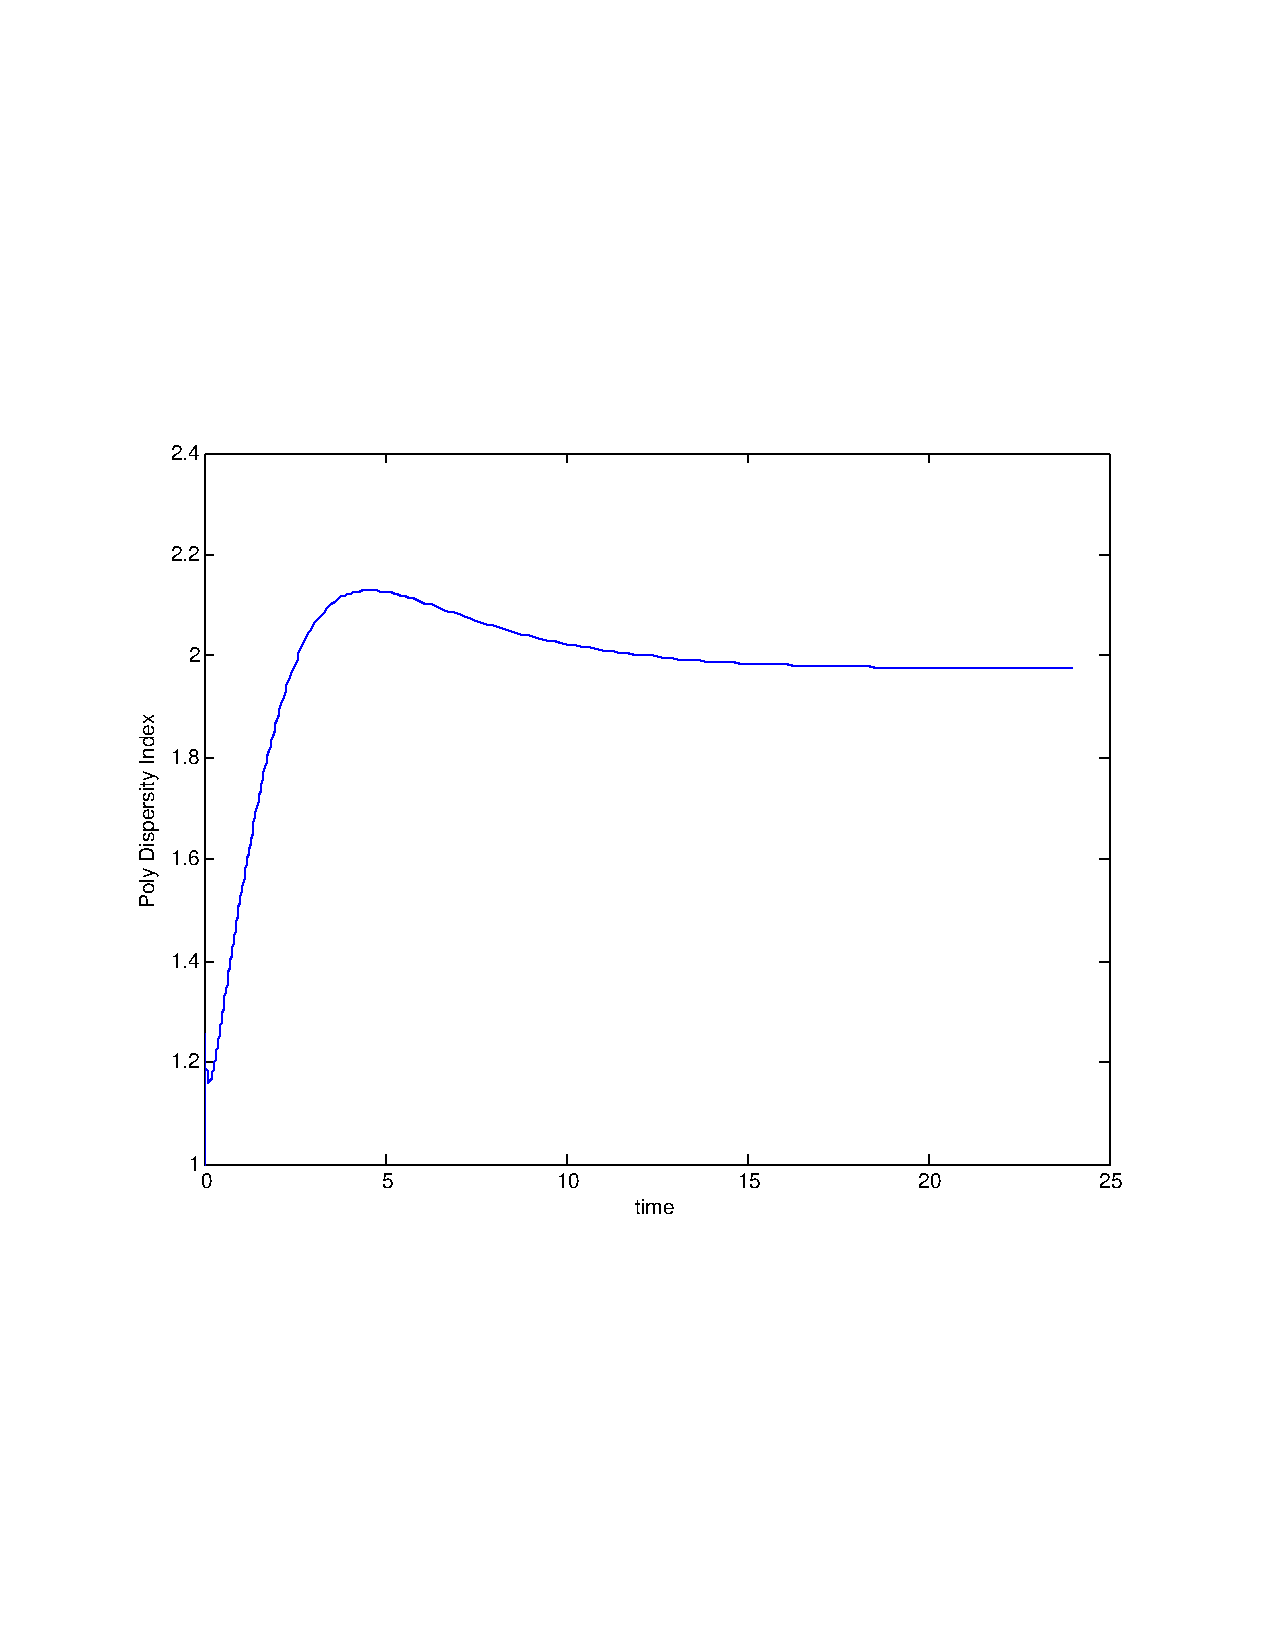
\includepdf{pdi.pdf}

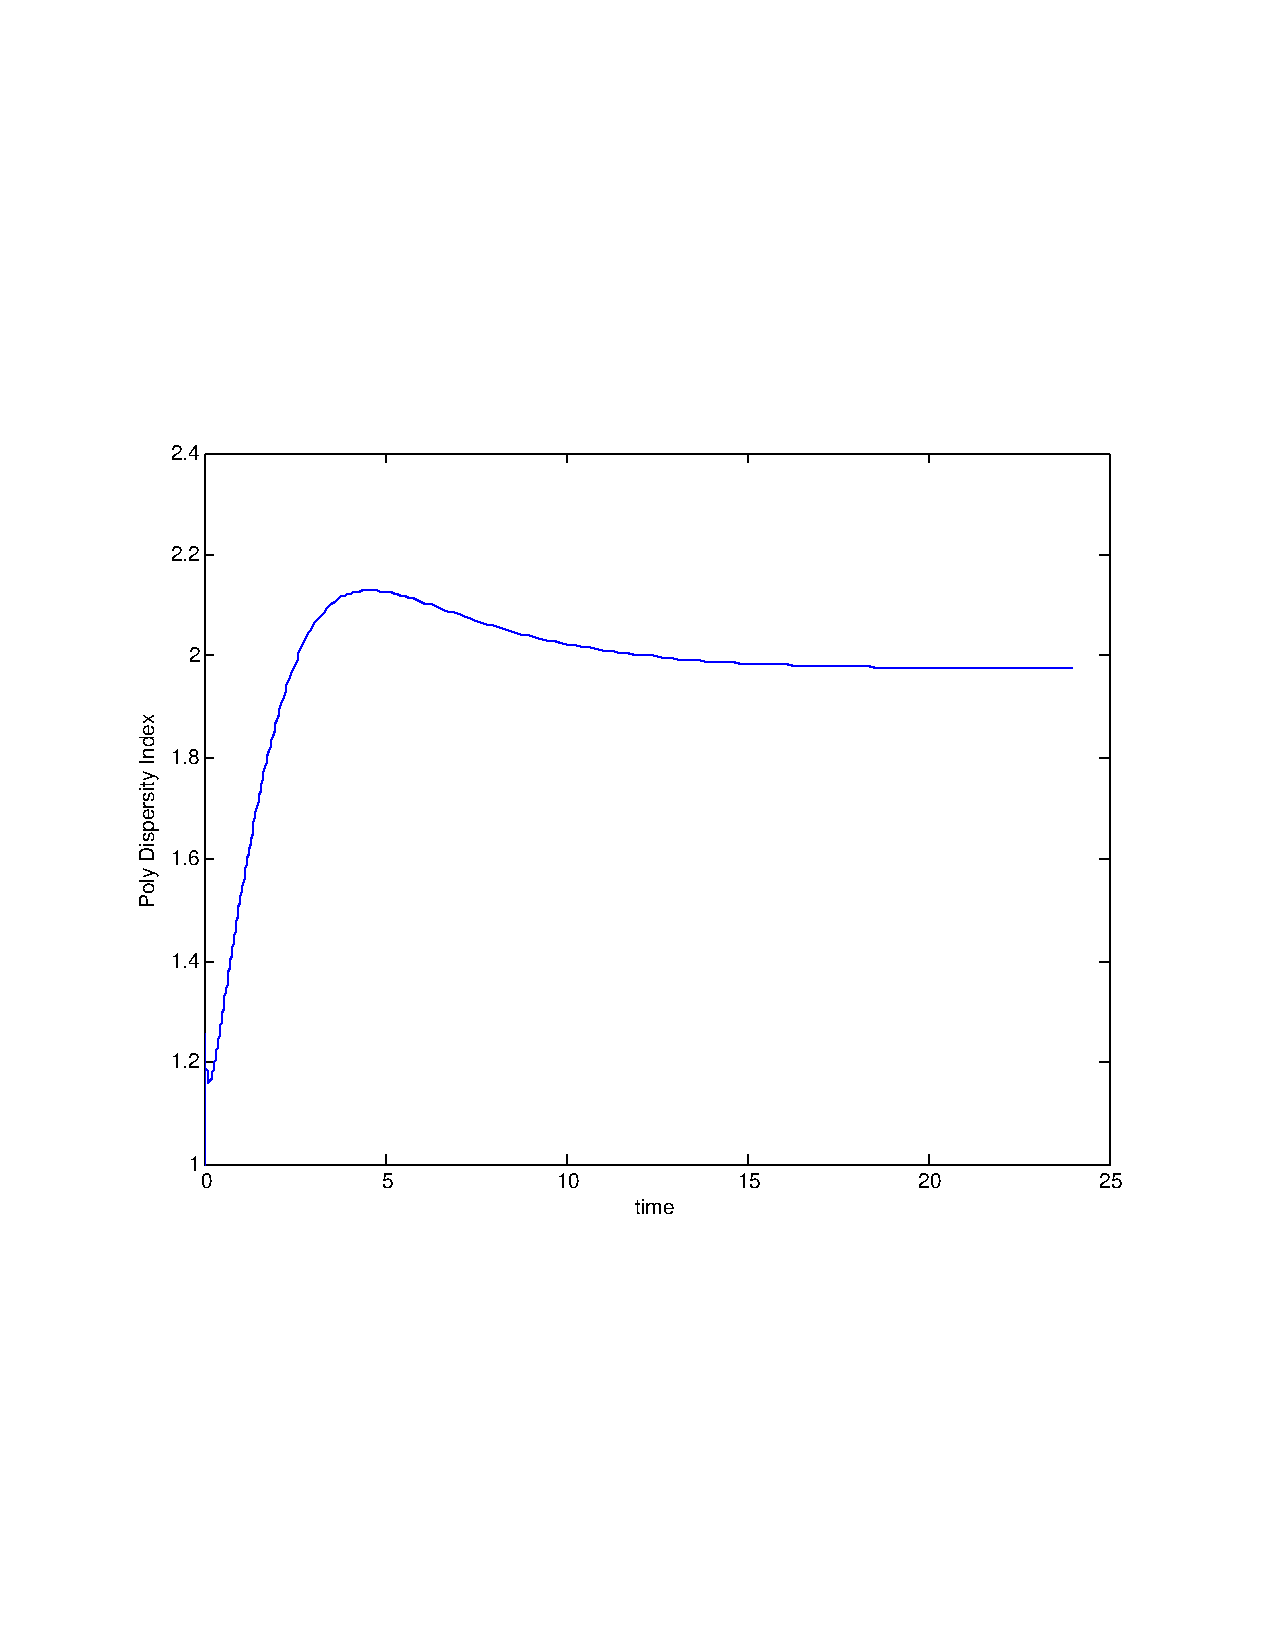
\includepdf{pdi.pdf}
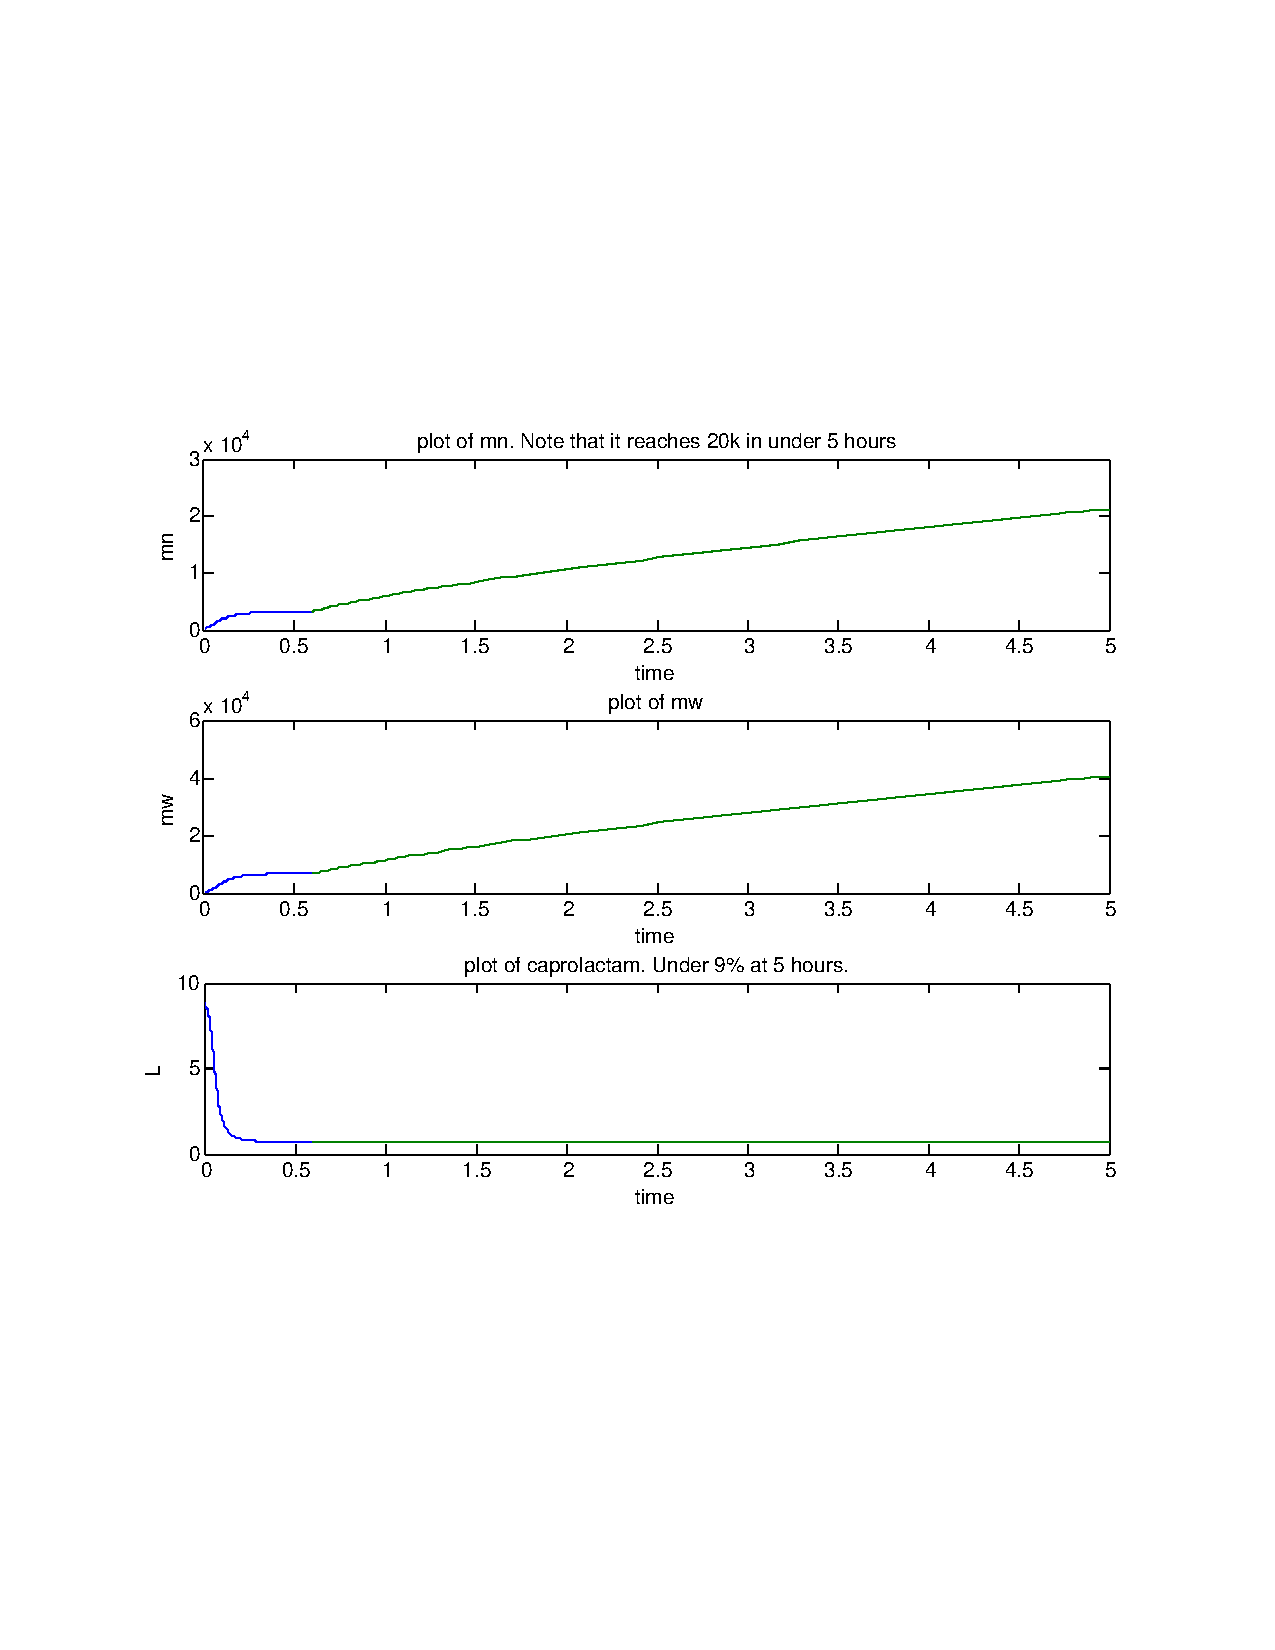
\includepdf{awesome.pdf}


\section*{Approach for part 2}

For obtaining an optimised process, I iterated over several possible reactions and stored the ones which satisfied the conditions, i.e final caprolactam concentration \textless 9\% and the final number averaged molecular weight should be greater than 20000.

We keep the initial conditions within a reasonable limit, temperature between 240 and 270 degrees celsius, a water concentration of 4 moles/litre and  P=0.1. The second reactor is running at 240 degrees celsius and has a water concentration of 0, which is reasonable assuming current dehumidifier technology.

After taking these conditions into account and making a second round of filtering, we then use a hit and trial method to find the appropriate timeline for both reactions. It is observed that the first reactor reaches equilibrium very quickly, so we can immediately transfer the contents to the second reactor.

These conditions are then taken into account when developing the final program.


\section*{Results}
\begin{enumerate}
\item Temperature for first reactor= 270 degrees celsius
\item Temperature for second reactor= 240 degrees celsius
\item Water for first reactor= 4 moles/litre
\item Water for second reactor= 0 moles/litre
\item time for first reactor= 0.6 hours
\item time for second reactor= 4.4 hours

\end{enumerate} 

    
\end{document}